
\documentclass[a4paper,punct=banjiao,twoside]{ctexrep}
% oneside/twoside 单面/双面打印适配版本.
% openright/openany 控制新的章节是否应该在奇数页的右侧开始, 但并不好用,建议手动插入空白页.
% fontset 设置字体集,可以选择的值包括 windows、mac、ubuntu 等,可以解决字体报错.
% punct=: 设置中文文档中的标点样式,可选的值包括 quanjiao 全角式:所有标点占一个汉字宽度,相邻两个标点占 1.5 汉字宽度;banjiao 半角式:所有标点占半个汉字宽度;kaiming 开明式:句末点号16用占一个汉字宽度,标号和句内点号占半个汉字宽度;等.


\usepackage[a4paper,hmargin={2.54cm,2.54cm},vmargin={3.175cm,3.175cm}]{geometry}
\headheight = 15 pt
%参见https://tex.stackexchange.com/questions/132170/what-do-headheight-headsep-etc-do-in-the-vmargin-package最高赞答案

\usepackage{amsmath,amssymb}
% 扩展支持的数学符号

\usepackage{mathrsfs}
% 引用


\usepackage[dvipsnames, svgnames, x11names]{xcolor}
% 扩展颜色

\usepackage[colorlinks=true,linkcolor=Maroon]{hyperref}
% 使用hyperref宏包, 对目录, 公式引用, 文献引用做超链接, 超链接方便电子版的阅读, 但不影响打印.
% pdfborder对超链接的边框大小进行设置, 模板中默认边框大小为0.
% colorlinks=true, 表示超链接对应的文字采用超链接边框的颜色, =false时保持原字体颜色.
% linkcolor=maroon, 设置超链接边框的颜色, 可以改为red,green等等.

\usepackage{amsthm}
% 配置定理环境
\theoremstyle{plain}
%plain(默认样式): 定理名称是正体,定理内容是斜体.
%definition: 定理名称和定理内容都是正体,其上下留有额外的空间.
%remark: 正体,其上下没有额外的空间.
\newtheorem{thm}{定理}[chapter]
% 如果需要在每一节中单独编号,请将[chapter]改为[section]
\newtheorem{lemma}[thm]{引理}
\newtheorem{axiom}[thm]{公理}
\newtheorem{coro}[thm]{推论}
\newtheorem{prop}[thm]{命题}
\newtheorem{con}[thm]{猜想}

\theoremstyle{definition}
\newtheorem{defn}[thm]{定义}
\newtheorem{asm}[thm]{假设}
\newtheorem{que}[thm]{问题}

\theoremstyle{remark}
\newtheorem{rem}{注}[chapter]
\newtheorem{example}{例}[chapter]
% 除了注和例之外,均是连续编号.
\renewcommand{\proofname}{\textbf{证明}}
% 如需将证毕符号改成黑色的正方形,请将下一行取消注释.
% \renewcommand{\qedsymbol}{$\blacksquare$}    
\newcommand{\dd}{\text{d}}
\newcommand{\R}{{\mathbb R}}
\newcommand{\N}{{\mathbb N}}
%\newcommand{\Z}{{\mathbb Z}}
%\newcommand{\C}{{\mathbb C}}
% 此处可以定义一些常用的记号,留给大家自由发挥咯,例如输入\dd 可以直接得到正体的d,用作积分号里dx中的d.

%其余的一些必要的宏包
\usepackage{xcolor,caption,array,enumerate}
\usepackage{graphicx} %插入图片的宏包
\usepackage{float} %设置图片浮动位置的宏包
\usepackage{subcaption} %插入多图时用子图显示的宏包

\usepackage{tikz}%画图
\usepackage{longtable, booktabs, threeparttable, caption, bicaption, multirow}
% 扩展表格功能
\usepackage[ruled,linesnumbered]{algorithm2e}
% 算法
\usepackage{listings}
\lstset{
  language=Python, % 设置语言
  basicstyle=\ttfamily, % 设置字体族
  breaklines=true, % 自动换行
  keywordstyle=\bfseries\color{NavyBlue}, % 设置关键字为粗体,颜色为 NavyBlue
  morekeywords={}, % 设置更多的关键字,用逗号分隔
  emph={self}, % 指定强调词,如果有多个,用逗号隔开
  emphstyle=\bfseries\color{Rhodamine}, % 强调词样式设置
  commentstyle=\itshape\color{black!50!white}, % 设置注释样式,斜体,浅灰色
  stringstyle=\bfseries\color{PineGreen!90!black}, % 设置字符串样式
  columns=flexible,
  numbers=left, % 显示行号在左边
  numbersep=2em, % 设置行号的具体位置
  numberstyle=\footnotesize, % 缩小行号
  frame=single, % 边框
  framesep=1em % 设置代码与边框的距离
}
% 自定义多级标题格式
%\CTEXsetup[nameformat={\huge \heiti},titleformat={\huge \heiti},beforeskip={0.0cm},afterskip={1.2cm}]{chapter}
% 上一行为旧版的语法,可以选择注释上一行,取消注释下一行.
\ctexset { chapter = { nameformat={\huge \heiti  },titleformat={\huge \heiti  },beforeskip={0.0cm},afterskip={1.2cm} } } 
\usepackage{titlesec}
\titleformat{\section}[block]{\Large\centering\heiti}{\arabic{chapter}.\arabic{section}}{1em}{}[]
\titleformat{\subsection}[block]{\large \heiti}{\arabic{chapter}.\arabic{section}.\arabic{subsection}}{1em}{}[]
\titleformat{\subsubsection}[block]{\normalsize\bfseries}{\arabic{subsection}-\alph{subsubsection}}{1em}{}[]
\titleformat{\paragraph}[block]{\small}{[\arabic{paragraph}]}{1em}{}[]
% 使用Ctex自带的\section的标题会出现问题,使用titlesec\chapter的标题要么无法显示汉字数字,要么无法显示字母A,只能做缝合怪了!

\usepackage{gbt7714}
% 将参考文献的格式更改为与国标《文后参考文献著录规则》GB/T 7714-2005一致.
% 需要使用其它格式时请将该行注释, 并在参考文献部分将指定语句取消注释.
\usepackage{tikz}


%导言区设置完毕
%%%%%%%%%%%%%%%%%%%%%%%%%%%%%%%%%%%%%%%%%%%%%%%%%%%%%%%%%%%%%%%%%%%%%%%%%%%%%%%%%%%%%%%%%%%%%%%%%%%%%%%%%%%%%%%%%%%%%%%%%%%%%%%%%%%%%%%%%%
\begin{document}
% 制作封面, 适用于研究生毕业论文.
%\begin{titlepage}
%    {
%        \hfill 
%        \footnotesize
%    \begin{tabular}{cc}
%        \makebox[4em][s]{学校代码}:&\makebox[5em][l]{10246}\\
%        \makebox[4em][s]{学号}:&\makebox[5em][l]{??300180???}\\
%
%    \end{tabular}
%    }
%    \vspace*{1.5cm}
%
%    \begin{center}
%        \begin{figure}[H] %H为当前位置,!htb为忽略美学标准,htbp为浮动图形
%            \centering %图片居中
%            
\includegraphics[width=0.46\textwidth]{figs/fudan-name.pdf} %插入图片,[]中设置图片大小,{}中是图片文件名
%            %\caption{Main name 0} %最终文档中希望显示的图片标题
%            \label{fudan-name} %用于文内引用的标签
%        \end{figure}
%        \vspace*{1.5cm}
%
%        \makebox[16em][s]{\LARGE{本科毕业论文}}
%        %(学术学位)
%        %若需要取消注释上一行,请相应改变下一行的行间距的取值
%        \vspace*{3cm}
%
%        {\bfseries \Large 论文题目}
%        \vspace*{1cm}
%
%        {\bfseries  English Title}
%        \vspace*{3cm}
%
%        \fontsize{14pt}{\baselineskip}\selectfont
%        \begin{tabular}{cc}
%            \makebox[6em][s]{院系}:&\makebox[8em][c]{数学科学学院}\\[1ex]
%            \makebox[6em][s]{专业}:&\makebox[8em][c]{数学与应用数学}\\[1ex]
%            \makebox[6em][s]{姓名}:&\makebox[8em][c]{XXX}\\[1ex]
%            %两个字姓名的同学可以将上一行改为
%            %\makebox[6em][s]{姓名}:&\makebox[3em][c]{XX}\\[1ex]
%            \makebox[6em][s]{指导老师}:&\makebox[8em][c]{XXX \ 教授}\\[1ex]
%            \makebox[6em][s]{完成日期}:&\makebox[8em][c]{\today}\\[1ex]
%        \end{tabular}     
%    \end{center}
%\end{titlepage}

\renewcommand{\thepage}{\roman{page}}

% 改写目录标题的格式
\renewcommand{\contentsname}{目\quad 录}
\tableofcontents
\setcounter{page}{1}

\chapter*{摘\quad 要}
\addcontentsline{toc}{chapter}{摘要}
\normalsize

这是我的中文摘要.

\chapter*{Abstract}
\addcontentsline{toc}{chapter}{Abstract}
\normalsize

This is my English abstract.

\noindent{\textbf{Keywords:}} 1; 2; 3\\
\noindent{\textbf{CLC code:}} O24

\clearpage
\mbox{}
\thispagestyle{empty}
% 为了保证第一章在奇书页.




\renewcommand{\thepage}{\arabic{page}}
\setcounter{page}{0}
% 论文的页码从正文重新开始计数












\chapter{引言}


双酚类物质(Bisphenols,BPs)是一种工业用化学物质, 被大量用于生产聚碳酸酯及环氧树脂\cite{3}. 这两种可能会含有BPs的高分子物质又常被投入生产食品接触材料或其他日常使用材料, 例如塑料杯,奶瓶,纸币,金属涂层等\cite{4}.在日常生活中, BPs通过皮肤渗透与口服摄入两种主要途径进入人体内环境,参与后续的分布与代谢.双酚A(BPA),作为最早投入工业生产的BPs,已被证实对人体具有毒性\cite{2}.事实上,BPA会对人体的多个系统(如呼吸系统,神经系统,生殖系统)造成损害\cite{5}.
BPA与双酚S(BPS)两种BPs经口服进入人体后, 经消化系统来到小肠,并在此分别葡萄糖醛酸化为BPA-g与BPS-g, 葡萄糖醛酸化后的双酚物质会进入血液循环并最终随尿液排出体外;未葡萄糖醛酸化的BPA或BPS将会进入肝脏并在此被部分磷酸化为BPA-s或BPS-s,部分BPs在肝脏仍会被葡萄糖醛酸化,这些衍生物与未发生反应的BPs都会直接进入血液循环并最终随尿液排出体外\cite{2,1}.同时,在小肠或肝脏处进入血液循环的BPs会随血液进入人体的各个器官,如脑,生殖腺等.若BPs经由皮肤渗透进入人体,将会直接进入血液循环并跟随血液到达各个器官,其中进入小肠或肝脏的部分BPs将会根据所处位置被葡萄糖醛酸化或是被磷酸化.
为了找寻比BPA更安全的替代品, 研究BPS等双酚物质在人体中的代谢过程是有必要的\cite{6}.

生理药代动力学模型(Physiology-Based Pharmacokinetic Model, PBPK)是药学中定量描述化学品在人体中吸收,分布,代谢,排泄过程的经典模型,常被用于化学品生态风险评价,人类健康风险评估以及药物开发\cite{7}.PBPK模型将包含血浆在内的对目标化学品特异性较强的靶点组织器官抽象为一个个”房室”,以质量守恒定律和相关生化反应为基础定量计算目标化学品在各房室之间的交换与各房室之内的代谢过程\cite{8}.当某些靶点组织器官的目标化学品含量难以实际测出时, PBTK模型的结果能够提供一个良好的预测 \cite{7}.只需要确定PBPK模型中重要参数的数值, 就能在脱离实际人体实验的情况下给出人体吸收目标化学品后靶点组织器官的化学品含量.

Yang等人在2015年首次建立了使用人类参数的BPA在生物体内的PBPK模型,该模型基于口服摄入的吸收方式, 共设置了10个仓室,分别为血浆,肝脏,脂肪,性腺,血流丰富组织,血流缓慢组织,大脑和皮肤,剩下两个仓室分别是BPA-g和BPA-s的反应仓室\cite{10}. Karrer等人在2018年重新调整了此PBPK模型, 提供了BPA的其他双酚类替代品的模型参数, 并增加了通过皮肤渗透吸收BPs的情形\cite{9}.Hu等人在2023年对皮肤渗透模型进行了改进,在原本皮肤作为单独仓室的基础上将其分割成了五个小仓室,分别为表皮储仓,角质层,活性表皮,毛囊以及未参与渗透吸收的未暴露皮肤\cite{11}.
该文章设置了志愿者实验, 利用BPS暴露后受试者尿液中BPS与BPS-g的含量来优化PBPK模型与皮肤仓室相关的三个参数, 并使用敏感性与不确定性分析评估了修改后的PBPK模型.

Hu等人文章的参数优化部分中使用了传统的优化算法, 在计算机上运行的时间较久. 本文将在其基础上利用神经网络模型对皮肤渗透吸收型PBPK模型内的三个目标参数做参数反演, 提升获取最优参数的速度的同时提高参数的准确性; 并利用数值实验来评估神经网络模型的效果.


\chapter{PBPK模型的建立}
Hu等人\cite{11}在github中共享了论文中的数据以及部分代码\cite{12}. 共享中包含了PBPK模型和参数优化所使用的受试者真实数据等, 本章内容参照了这些工作.该模型对多种双酚类物质都适用, 本文后续只讨论
双酚S(BPS)的情形, 且只考虑皮肤暴露途径的外源BPS输入.
\section{模型的实验与生理背景}
Hu\cite{11}等人通过使用含有氘代BPS(BPS-d8)的热敏纸摩擦手指的方式令受试者暴露于BPS.受试者接触热敏纸共$\frac{1}{6}h$, 脱离热敏纸后再等待$2h$, $\frac{13}{6}h$时彻底清洗皮肤,清空表皮储仓内的BPS.
在接触实验开始的$72h$, 受试者被要求每$4.3h$左右提供一次尿液样本, 以检测尿液中的BPS与BPS-g的含量.
在另一个BPS人体接触实验中, Khmiri等人\cite{13}同时监测了受试者的血液与尿液. 接触BPS起的前$2h$内每$0.25h$取样一次血液, 第2小时至第8小时内每$1h$取样一次血液, 之后分别在$10h$, $24h$, $48h$时取样一次血液.
尿液的取样节点不是固定的, 而是将接触BPS后$48h$分成了11个时段. 受试者在单个时段内的所有排尿都会被收集,作为该时段标签下的一个整体取样. 

从受试者与热敏纸接触时起, 热敏纸内的BPS通过手指表皮储存进入毛囊和角质层, 接着扩散进入活性表皮层, 再通过毛囊和活性表皮层与内环境的交换进入体循环, 平行分层皮肤仓室内的物质交换情况的图片形式如图\ref{分层皮肤}. 血浆携带BPS通过血液交换将
其送入肝脏, 脑, 脂肪, 性腺等组织器官. 部分BPS在肝脏反应为BPS-g或BPS-s.体内的BPS-g与BPS-s不会再反应为其他物质, 这两种物质
会像始终未发生反应的BPS一样, 最终随血液进入肾脏, 通过尿液排出. 在只有皮肤暴露途径吸收外源BPS的情况下, 不考虑BPS的肝肠循环过程, 认为胃肠部不存在BPS, 且小肠不发生BPS葡萄苷酸化为BPS-g的反应. 
\begin{figure}[H]
  \centering
  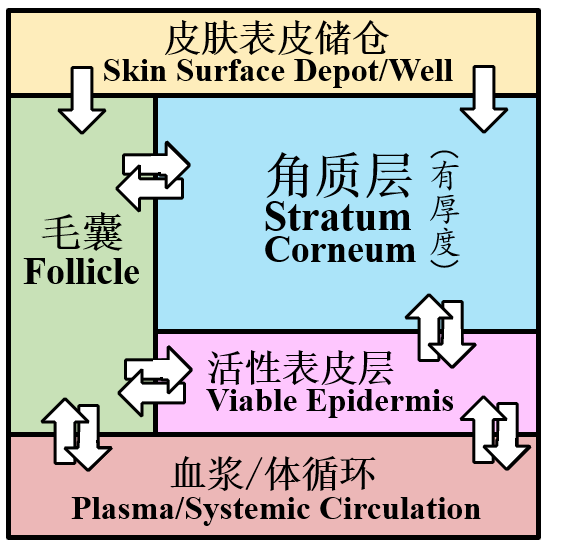
\includegraphics[scale=0.6]{./figs/p1.png}
  \caption{平行分层皮肤仓室的简化图解(箭头代表BPS的可能运输方向)}
  \label{分层皮肤}
\end{figure}

 
\section{模型的数学形式}
本文中的PBPK模型共有个14仓室,包括:暴露皮肤\{皮肤表皮储仓, 角质层, 毛囊, 活性表皮层\}, 胃, 小肠, 未暴露于化学品的皮肤, 血浆, 脂肪, 性腺, 肝脏, 脑, 血流丰富组织, 血流缓慢组织.
其中暴露的含义为“在实验中与BPS接触”.
根据各仓室之间的关系以及BPS在各仓室内的生化反应, 得到19个解关于时间$t$变化的常微分方程与1个偏微分方程. 这些微分方程共同构成了BPS的带平行分层皮肤仓室的PBPK模型.  

\subsubsection*{角质层内BPS的浓度$\varphi(x,t)$}
如(\ref{eq0}), 其中的偏微分方程本质上是一个扩散对流方程,其解$\varphi$代表角质层(Stratum Corneum)中BPs含量, 自变量$x$代表角质层的深度, 自变量$t$代表时间, $DSC$代表BPS在角质层中的有效扩
散系数$(cm^2/h)$, $u_1$代表BPS随脱屑向皮肤表面转移的速度$(cm/min)$, $T_{SC}$代表角质层的深度$(um)$, $HSC_{well}$代表角质层和皮肤表皮储仓之间的分配系数, 
$C_{well}(t)$代表皮肤表皮储仓在t时刻的BPS浓度$(nmol/cm^3)$, $HSC_{VE}$代表角质层和活性表皮之间的分配系数, $C_{VE}(t)$代表活性表皮在t时刻的BPS浓度$(nmol/cm^2)$.

\begin{equation}\label{eq0}
  \left\{\begin{aligned}
    \frac{\partial \varphi(x,t) }{\partial t^2} &= DSC \frac{\partial^2 \varphi(x,t)}{\partial x^2} + u_1 \frac{\partial \varphi(x,t)}{\partial t}, && 0\leq x \geq T_{SC}, \quad t\geq 0\\
    \varphi(0,t) &= HSC_{well} \times C_{well}(t), &&t\geq 0\\
    \varphi(T_{SC},t) &= HSC_{VE} \times C_{VE}(t), &&t\geq 0\\
    \varphi(x,0) &= 0, &&0\leq x \geq T_{SC}\\
  \end{aligned}\right.
  \end{equation}
\noindent 使用空间离散化的办法, 将角质层视作一个长度为$T_{SC}$的线段, 将该线段等距分为$10$段, 共$11$个节点$\{x_i\}_{0\leq i\leq 10}$. 其中第一个节点$x_0$视作皮肤表皮储仓, 最后一个节点$x_{10}$视作活性表皮.
$x_1$至$x_9$九个节点处BPS浓度的一阶与二阶空间导数值通过中心差分法近似表示: 
\begin{equation}\label{eq1.1}
  \left\{\begin{aligned}
    \frac{\partial^2}{\partial x^2}\varphi(x_j, t) &\approx \frac{\varphi_{j+1}(t) - 2\varphi_j(t) + \varphi_{j-1}(t)}{(\Delta x)^2}\\
    \frac{\partial}{\partial x}\varphi(x_j, t) &\approx \frac{\varphi_{j+1}(t) - \varphi_{j-1}(t)}{2\Delta x}\\
  \end{aligned}\right.
  \end{equation}
  \noindent 整理后得到这九个节点处BPS浓度关于时间的一阶导数值如(\ref{eq1}), $i=2,3,\dots,8$与(\ref{eq2}),(\ref{eq3}).其中$SCDX = \frac{T_{SC}}{10}$, 
  $V_{well}$为暴露皮肤表面储仓沉积体积$(cm^3)$, $A_{well}(t)$为皮肤表皮储仓在t时刻的BPS含量$(nmol)$,$V_{TVE}$为暴露皮肤活性表皮层体积$(cm^3)$, $A_{VE}(t)$为活性表皮在t时刻的BPS含量$(nmol)$.
  节点$x_1$和$x_9$处的时间导数值与其他节点不同的原因是: 与它们相邻的部分涉及到皮肤的不同层室,需要利用BPS在不同层室组织间
  的分配系数来确定两个不同层室间BPS的转移情况. 
\begin{equation}\label{eq1}
  \frac{dC_{SCi}(t)}{dt}=\left(\frac{DSC}{SCDX^2} -\frac{u_1}{2 \times  SCDX}\right)C_{SCi-1}(t)-\frac{2 \times DSC}{SCDX^2}  C_{SCi}(t)+\left(\frac{DSC}{SCDX^2}+\frac{u_1}{2 \times  SCDX}\right)C_{SCi+1}(t).
\end{equation}

\begin{multline}\label{eq2}
  \frac{dC_{SC1}(t)}{dt}=\left(\frac{DSC \times  HSC_{well}}{V_{well}  \times  SCDX^2 }-\frac{u_1  \times  HSC_{well}}{V_{well}  \times  2 \times  SCDX}\right)A_{well}(t)   -\frac{2 \times DSC}{SCDX^2}  C_{SC1}(t)\\
  +\left(\frac{DSC}{SCDX^2}+\frac{u_1}{2 \times  SCDX}\right)C_{SC2}(t).
\end{multline}

\begin{multline}\label{eq3}
  \frac{dC_{SC9}(t)}{dt}=\left(\frac{DSC}{SCDX^2} -\frac{u_1}{2 \times  SCDX}\right)C_{SC8}(t)-\frac{2 \times DSC}{SCDX^2}  C_{SC9}(t)\\
  +\left(\frac{DSC \times  HSC_{VE}}{V_{TVE}  \times  SCDX^2 }-\frac{u_1  \times  HSC_{VE}}{V_{TVE}  \times  2 \times  SCDX}\right)A_{VE}(t) .
\end{multline}

接下来介绍模型中余下的19个解关于时间$t$变化的常微分方程, 此部分内方程中出现的变量与常量的含义详情见附录\ref{app:B}.
\subsubsection*{毛囊内BPS的含量$A_{Fo}(t)$}
见(\ref{eq10}), 方程等式两端为$A_{Fo}(t)$的一阶导数. 在该PBPK模型中, 毛囊与皮肤表皮储仓和血液之间有着直接的物质交换, 故毛囊内BPS含量的增减与表皮储仓或血浆中BPS的含量有关, BPS在宏观上遵循着顺浓度梯度运输的
规则在不同组织内交换. 同时, 毛囊内BPS含量的增减会受到自身的限制, 当毛囊内BPS浓度高于血浆或表皮储仓中BPS浓度时, BPS会顺浓度梯度进入浓度小的组织.
\begin{multline}\label{eq10}
  \frac{dA_{Fo}(t)}{dt} = -\left(\frac{Pfo \times  AEXP \times  FEXP}{V_{TFo}  \times  HFo_{well} }
  +\frac{Qskin \times  AEXP \times  0.25}{BSA \times  V_{TFo}  \times  pskin}\right)A_{Fo}(t)\\
  +\frac{Pfo \times  AEXP \times  FEXP}{V_{well}  }A_{well}(t)+\frac{Qskin \times  AEXP \times  0.25}{BSA \times  V_{plasma}} A_{plasma}(t).
\end{multline}

\subsubsection*{皮肤表皮储仓内BPS的含量$A_{well}(t)$}
见(\ref{eq11}), 方程等式两端为$A_{well}(t)$的一阶导数. 类似(\ref{eq10}), 等式右端表现出了表皮储仓与节点$x_1$处的角质层和毛囊之间的顺浓度梯度物质交换关系. 同时, 皮肤表皮储存作为在实验
中直接和外源BPS接触的部位, 它要接受一个剂量为$f_1 (t)$(单位:nmol)的持续的外源BPS输入. 当$t>Time_{add}=\frac{1}{6}h$时, 皮肤停止接触外源BPS, $f_1 (t)=0$. 
等式右端有一个因数$ON(t)$, 当$t\leq Time_{expose}=\frac{13}{6}h$时, $ON(t)=1$, 皮肤处于BPS暴露状态;当$t> Time_{expose}$时, $ON(t)=0$, 暴露过BPS的皮肤被彻底清洗, 表皮储仓清空, 后续$A_{well}(t)$的值与一阶
导数值都为0.
\begin{multline}\label{eq11}
  \frac{dA_{well}(t)}{dt} = \left(\frac{DSC \times  AEXP \times  (1-FEXP)}{SCDX} C_{SC1}(t)-\frac{Pfo \times  AEXP \times  FEXP}{V_{TFo} \times  HFo_{well}} A_{Fo}(t)\right.\\
  \left. -\left(\left(\frac{DSC \times  HSC_{well}}{V_{well} \times  SCDX}-\frac{u_1 \times  HSC_{well}}{V_{well} }\right) \times  AEXP \times  (1-FEXP) \right.\right.\\
  \left.\left.-\frac{Pfo \times  AEXP \times  FEXP}{V_{well}} \right)A_{well}(t)+f_1 (t) \right) \times  ON(t).
\end{multline}

\subsubsection*{活性表皮层内BPS的含量$A_{VE}(t)$}
见(\ref{eq12}), 方程等式两端为$A_{VE}(t)$的一阶导数. 类似(\ref{eq10}), 等式右端表现出了活性表皮层与节点$x_9$处的角质层, 毛囊和血浆之间的顺浓度梯度物质交换关系. 
\begin{multline}\label{eq12}
  \frac{dA_{VE}(t)}{dt}=\frac{DSC \times  AEXP \times  (1-FEXP)}{SCDX} C_{SC9}(t)+\left(\left(\frac{-DSC \times  HSC_{VE}}{V_{TVE}  \times  SCDX}-\frac{u_1  \times  HSC_{VE}}{V_{TVE} }\right)\times \right.\\ 
   \left.AEXP \times  (1-FEXP)-\frac{Qskin \times  AEXP \times  0.75}{BSA \times  V_{TVE}  \times  pskin}\right)A_{VE}(t)+\frac{Qskin \times  AEXP \times  0.75}{BSA \times  V_{plasma} } A_{plasma}(t).
\end{multline}

\subsubsection*{胃部BPS的含量$A_{ST}(t)$}
见(\ref{eq13}), 方程等式两端为$A_{ST}(t)$的一阶导数. 等式右端的第一个加数代表胃部BPS向肝脏和小肠转移的过程, 第二个加数是剂量为$f_2 (t)$(单位:nmol)的通过口服吸收的外源BPS. 但由于本文不考虑
口服吸收BPS的情形, $f_2 (t)\equiv 0$, 可认为胃部内始终不含有BPS或它的衍生物.
\begin{equation}\label{eq13}
  \frac{dA_{ST}(t)}{dt}=-(k_0+ge)A_{ST}(t)+f_2 (t).
\end{equation}
\subsubsection*{未暴露于BPS的皮肤, 脂肪, 性腺, 脑部, 血流丰富组织, 血流缓慢组织的BPS的含量}
见(\ref{eq14})至(\ref{eq20}), 方程等式两端为小标题中组织器官内BPS含量的一阶导数. 这些等式的右端一致地代表了对应组织器官与血浆之间的顺浓度梯度物质交换关系. 
\begin{multline}\label{eq14}
  \frac{dA_{skin}(t)}{dt}=\frac{-Qskin \times  (1-\frac{AEXP}{BSA})}{(V_{skin}-V_{TSC}-V_{TVE}-V_{TFo}) \times  pskin} A_{skin}(t)+\frac{Qskin \times  (1-\frac{AEXP}{BSA})}{V_{plasma}}  A_{plasma}(t).
\end{multline}

\begin{equation}\label{eq15}
  \frac{dA_{fat}(t)}{dt}=\frac{-Qfat}{V_{fat}  \times  pfat} A_{fat}(t)+\frac{Qfat}{V_{plasma}}  A_{plasma}(t).
\end{equation}

\begin{equation}\label{eq16}
  \frac{dA_{gonad}(t)}{dt}=\frac{-Qgonad}{V_{gonad}  \times  pgonad} A_{gonad}(t)+\frac{Qgonad}{V_{plasma}}  A_{plasma}(t).
\end{equation}

\begin{equation}\label{eq18}
  \frac{dA_{brain}(t)}{dt}=\frac{-Qbrain}{V_{brain}  \times  pbrain} A_{brain}(t)+\frac{Qbrain}{V_{plasma}}  A_{plasma}(t).
\end{equation}

\begin{equation}\label{eq19}
  \frac{dA_{rich}(t)}{dt}=\frac{-Qrich}{V_{rich}  \times  prich} A_{rich}(t)+\frac{Qrich}{V_{plasma}}  A_{plasma}(t).
\end{equation}

\begin{equation}\label{eq20}
  \frac{dA_{slow}(t)}{dt}=\frac{-Qslow}{V_{slow}  \times  pslow} A_{slow}(t)+\frac{Qslow}{V_{plasma}}  A_{plasma}(t).
\end{equation}

\subsubsection*{血浆内的BPS的含量}
见(\ref{eq17}), 方程等式两端为血浆内BPS含量的一阶导数. 血浆是体循环的重要组成部分, 该PBPK模型内的各仓室由血浆连接起来, 几乎每个仓室都与血浆有直接的物质交换, BPS从组织器官内进入血浆, 血浆又
携带着BPS进入各个组织器官. 等式的右端代表了血浆与毛囊, 活性表皮层, 未直接暴露于BPS的皮肤组织, 脂肪, 性腺, 脑部, 血流丰富组织, 血流缓慢组织, 肝脏之间的顺浓度梯度物质交换关系. 
等式右端除了$A_{plasma}(t)$项外每一项都有因数$Qc-Kurinebps$, 其中$Qc$是心脏血流速度$(L/h)$, $Kurinebps$是BPS的尿液排泄参数$(L/h)$, 它们相减代表了每轮血液循环净剩的携带了BPS的血浆量.
\begin{multline}\label{eq17}
  \frac{dA_{plasma}(t)}{dt}=\frac{(Qc-Kurinebps) \times  Qskin \times  \frac{AEXP}{BSA} \times  0.25}{Qc \times  V_{TFo}  \times  pskin} A_{Fo}(t)\\
  +\frac{(Qc-Kurinebps) \times  Qskin \times  \frac{AEXP}{BSA} \times  0.75}{Qc \times  V_{TVE}  \times  pskin} A_{VE}(t)\\
  +\frac{(Qc-Kurinebps) \times  Qskin \times  (1-\frac{AEXP}{BSA})}{Qc \times  (V_{skin}-V_{TSC}-V_{TVE}-V_{TFo}) \times  pskin} A_{skin}(t)\\
  +\frac{(Qc-Kurinebps) \times  Qfat}{Qc \times  V_{fat}  \times  pfat} A_{fat}(t)
  +\frac{(Qc-Kurinebps) \times  Qgonad}{Qc \times  V_{gonad}  \times  pgonad} A_{gonad}(t)\\
  -\frac{Qc}{V_{plasma}}  A_{plasma}(t)+\frac{(Qc-Kurinebps) \times  Qbrain}{Qc \times  V_{brain} \times  pbrain} A_{brain}(t)\\
  +\frac{(Qc-Kurinebps) \times  Qrich}{Qc \times  V_{rich}  \times  prich} A_{rich}(t)
  +\frac{(Qc-Kurinebps) \times  Qslow}{Qc \times  V_{slow}  \times  pslow} A_{slow}(t)\\
  +\frac{(Qc-Kurinebps) \times  Qliver}{Qc \times  V_{liver} \times  pliver} A_{liver}(t).
\end{multline}

\subsubsection*{胃肠部的BPS-g的含量$A_{GIBPSg}(t)$与胃肠部的BPS-s的含量$A_{GIBPSs}(t)$}
见(\ref{eq21}), 方程等式两端为胃肠部的BPS-g的含量的一阶导数. 等式右端的第二个加数代表了小肠内的BPS葡萄苷酸化为BPS-g的过程, 第一个加数代表了BPS-g从胃肠部进入血液的过程. 
在本文中, 没有口服吸收途径, 认为胃肠部不存在BPS-g或BPS-s. 对于(\ref{eq22})有类似的说明, 不同在于小肠内几乎不发生BPS硫酸盐化为BPS-s的反应.
\begin{equation}\label{eq21}
  \frac{dA_{GIBPSg}(t)}{dt}=-kGIing \times  A_{GIBPSg}(t)+\frac{Vmaxgutg \times  A_{SI}(t)}{enterocytes \times  Kmgutg+A_{SI}(t)+\frac{A_{SI}(t)^2}{enterocytes \times  Ksigutg}}.
\end{equation}

\begin{equation}\label{eq22}
  \frac{dA_{GIBPSs}(t)}{dt}=-kGIins \times  A_{GIBPSs}(t)+\frac{Vmaxguts \times  A_{SI}(t)}{enterocytes \times  Kmguts+A_{SI}(t)}.
\end{equation}
\subsubsection*{小肠的BPS的含量$A_{SI}(t)$}
见(\ref{eq23}), 方程等式两端为小肠的BPS的含量的一阶导数. 等式右端的第一个加数代表了口服BPS时胃部BPS进入小肠的过程, 第二个加数代表了小肠内部分BPS进入肝脏的过程, 后两个加数代表了部分BPS在小肠内葡萄苷酸化为BPS-g与硫酸盐化为BPS-s的反应过程
(小肠内几乎不发生BPS磷酸盐化反应, 此处对应的最大反应速率$Vmaxguts$非常小). 
在本文中, 没有口服吸收BPS的途径, 认为小肠内不存在BPS及其衍生物. 
\begin{multline}\label{eq23}
  \frac{dA_{SI}(t)}{dt}=ge \times  A_{ST}(t)-k1 \times  A_{SI}(t)-\frac{Vmaxgutg \times  A_{SI}(t)}{enterocytes \times  Kmgutg+A_{SI}(t)+\frac{A_{SI}(t)^2}{enterocytes \times  Ksigutg}}\\
  -\frac{Vmaxguts \times  A_{SI}(t)}{enterocytes \times  Kmguts+A_{SI}(t)}.
\end{multline}
\subsubsection*{肝脏的BPS的含量$A_{liver}(t)$}
见(\ref{eq24}), 方程等式两端为肝脏的BPS的含量的一阶导数. 等式右端的前两个加数分别代表了口服BPS时胃部和小肠内BPS进入肝脏的过程, 第三第四个加数代表了肝脏与血浆之间的顺浓度梯度物质交换关系, 第五第六个加数代表了
BPS-g与BPS-s引起肝脏内部分BPS发生肝肠循环的过程, 后两个加数代表了部分BPS在肝脏内葡萄苷酸化为BPS-g与硫酸盐化为BPS-s的反应过程. 
\begin{multline}\label{eq24}
  \frac{dA_{liver}(t)}{dt}=k0 \times  A_{ST}(t)+k1 \times  A_{SI}(t)+\frac{Qliver}{V_{plasma} } A_{plasma}(t)-\frac{Qliver}{V_{liver}  \times  pliver} A_{liver}(t)\\
  +kenterobpsg \times  A_{BPSg\_delay}(t)+kenterobpss \times  A_{BPSs\_delay}(t)\\
  -\frac{Vmaxliverg \times  A_{liver}(t)}{V_{liver}  \times  pliver \times  Kmliverg+A_{liver}(t)}-\frac{Vmaxlivers \times  A_{liver}(t)}{V_{liver}  \times  pliver \times  Kmlivers+A_{liver}(t)}.
\end{multline}

\subsubsection*{发生肝肠循环/小肠内的BPS-g/BPS-s的量$A_{BPSg\_delay}(t)$/$A_{BPSs\_delay}(t)$}
见(\ref{eq25}), 方程等式两端为发生肝肠循环的BPS-g的量的一阶导数. 等式右端的第一个加数代表了胃肠部BPS-g进入血浆后再进入肝肠循环的过程,第二个加数代表了肝肠循环中的BPS-g进入血液循环的过程, 最后一个加数
代表了肝脏中BPS新转化成的BPS-g进入肝肠循环的过程. 对于发生肝肠循环的BPS-s的量的方程(\ref{eq26}), 有着完全一致的描述.
\begin{multline}\label{eq25}
  \frac{dA_{BPSg\_delay}(t)}{dt}=met2g \times  kGIing \times  A_{GIBPSg}(t)-(kentero+k4_{IV}+kenterobpsg) \times  A_{BPSg\_delay}(t)\\
  +\frac{met2g \times  Vmaxliverg \times  A_{liver}(t)}{V_{liver}  \times  pliver \times  Kmliverg+A_{liver}(t)}.
\end{multline}

\begin{multline}\label{eq26}
  \frac{dA_{BPSs\_delay}(t)}{dt}=met2s \times  kGIins \times  A_{GIBPSs}(t)-(kentero+k4_{IV}+kenterobpss) \times  A_{BPSs\_delay}(t)\\
  +\frac{met2s \times  Vmaxlivers \times  A_{liver}(t)}{V_{liver}  \times  pliver \times  Kmlivers+A_{liver}(t)}.
\end{multline}

\subsubsection*{人体内BPS-g/BPS-s的总含量$A_{BPSg}(t)$/$A_{BPSs}(t)$}
见(\ref{eq27}), 方程等式两端为人体内BPS-g的总含量的一阶导数. 等式右端的第一个加数代表了口服摄入BPS时, 胃肠部产生的BPS-g进入血液后未进入肝肠循环的部分BPS-g, 第二个加数代表了正在进行肝肠循环的BPS-g, 第三个
加数代表了BPS-g随尿液排出人体的过程, 最后一个加数代表了BPS通过肝脏转化成的BPS-g进入血液后未进入肝肠循环的部分BPS-g.(\ref{eq28})与之相似.

\begin{multline}\label{eq27}
  \frac{dA_{BPSg}(t)}{dt}=met1g \times  kGIing \times  A_{GIBPSg}(t)+kentero \times  A_{BPSg\_delay}(t)-\frac{Kurinebpsg}{Vbodyg+10^{-34} } A_{BPSg}(t)\\
  +\frac{met1g \times  Vmaxliverg \times  A_{liver}(t)}{V_{liver}  \times  pliver \times  Kmliverg+A_{liver}(t)}.
\end{multline}

\begin{multline}\label{eq28}
  \frac{dA_{BPSs}(t)}{dt}=met1s \times  kGIins \times  A_{GIBPSs}(t)+kentero \times  A_{BPSs\_delay}(t)-\frac{Kurinebpss}{Vbodys+10^{-34}} A_{BPSs}(t)\\
  +\frac{met1s \times  Vmaxlivers \times  A_{liver}(t)}{V_{liver}  \times  pliver \times  Kmlivers+A_{liver}(t)}.
\end{multline}


\section{PBPK模型的求解}
确定模型的数学形式后, 将Hu等人\cite{12}提供的数据相对应地代入至方程的各个参数, 使用Python中的第三方库函数scipy.integrate.odeint()对微分方程组求解. 
每个方程的解都对应了一条人体某组织器官或尿液内BPS(或BPS-g, BPS-s)含量随时间变化的曲线, 故每个解的初值都应设置为0
\clearpage
\mbox{}
\thispagestyle{empty}

\appendix
% 附录部分
\chapter{代码}
\section{代码环境}
\begin{lstlisting}[language=PYTHON]

\end{lstlisting}
\chapter{PBPK模型物理量名称-含义对照表}
\CTEXsetup[format={\Large\bfseries}]{section}
\section*{模型中待求解变量}
\label{app:B}
\noindent$C_{SCi}(t)$  {\hfill 暴露皮肤组织的深度为$i\times \frac{T_{SC}}{10}$的角质层在t时刻的BPS浓度$(nmol/cm^3)$}\\
$A_{Fo}(t)$ {\hfill  暴露皮肤组织的毛囊在t时刻的BPS含量$(nmol)$}\\
$A_{well}(t)${\hfill 暴露皮肤组织的表皮储仓在t时刻的BPS含量$(nmol)$}\\
$A_{VE}(t)${\hfill 暴露皮肤组织的活性表皮在t时刻的BPS含量$(nmol)$}\\
$A_{ST}(t)${\hfill 胃部在t时刻的BPS含量$(nmol)$}\\
$A_{skin}(t)${\hfill 未暴露皮肤组织在t时刻的BPS含量$(nmol)$}\\
$A_{fat}(t)${\hfill 脂肪组织在t时刻的BPS含量$(nmol)$}\\
$A_{gonad}(t)${\hfill 性腺在t时刻的BPS含量$(nmol)$}\\
$A_{plasma}(t)${\hfill 血浆在t时刻的BPS含量$(nmol)$}\\
$A_{brain}(t)${\hfill 脑部在t时刻的BPS含量$(nmol)$}\\
$A_{rich}(t)${\hfill 血流丰富组织在t时刻的BPS含量$(nmol)$}\\
$A_{slow}(t)${\hfill 血流缓慢组织在t时刻的BPS含量$(nmol)$}\\
$A_{GIBPSg}(t)${\hfill 胃肠部在t时刻的BPS-g含量$(nmol)$}\\
$A_{GIBPSs}(t)${\hfill 胃肠部在t时刻的BPS-s含量$(nmol)$}\\
$A_{SI}(t)${\hfill 小肠在t时刻的BPS含量$(nmol)$}\\
$A_{liver}(t)${\hfill 肝脏在t时刻的BPS含量$(nmol)$}\\
$A_{BPSg\_delay}(t)${\hfill 发生了肝肠循环的BPS-g的量/小肠在t时刻的BPS-g含量$(nmol)$}\\
$A_{BPSs\_delay}(t)${\hfill 发生了肝肠循环的BPS-s的量/小肠在t时刻的BPS-s含量$(nmol)$}\\
$A_{BPSg}(t)${\hfill 整个机体在t时刻的BPS-g含量$(nmol)$}\\
$A_{BPSs}(t)${\hfill 整个机体在t时刻的BPS-s含量$(nmol)$}

\section*{其他变量}
\noindent$\varphi(x,t)${\hfill   暴露皮肤组织的角质层深度x处在t时刻的BPS浓度$(nmol/cm^3)$,}\\
$f_1(t)$ {\hfill  皮肤接触外源BPS的量$(nmol)$, 当$t> Time_{add}$时, $f_1(t)=0$}\\
$ON(t)$ {\hfill  布尔值, 当$t\leq Time_{expose}$时, $ON(t)=1$, 皮肤处于BPS暴露状态;}\\ 
.\hfill 当$t> Time_{expose}$时, $ON(t)=0$, 皮肤处于未暴露状态\\
$f_2(t)$ {\hfill  口服外源BPS的量$(nmol)$, 本文中不考虑口服情况, $f_2(t)=0$}\\

\section*{待反演的参数}
\noindent$DSC$ {\hfill  角质层中的有效扩散系数$(cm^2/h)$}\\
$u_1$ {\hfill  由脱屑而向皮肤表面转移的速度$(cm/min)$}\\
$Pfo$ {\hfill  毛囊的渗透系数$(cm/h)$}

\section*{理化数据中的常量}
\noindent$T_{SC}$ {\hfill  角质层的深度$(um)$}\\
$SCDX$ {\hfill  角质层的深度的$\frac{1}{10}(um)$}\\
$HSC_{well}$ {\hfill  角质层和皮肤表皮储仓之间的分配系数}\\
$V_{well}$ {\hfill  暴露皮肤组织的表面储仓体积$(L)$}\\
$HSC_{VE}$ {\hfill  角质层和活性表皮之间的分配系数}\\
$V_{TVE}$ {\hfill  暴露皮肤组织的活性表皮层体积$(L)$}\\
$AEXP $ {\hfill  暴露皮肤组织面积$ (dm^2)$}\\
$ FEXP$ {\hfill  暴露皮肤组织中毛囊的面积分数}\\
$HFo_{well}$ {\hfill  毛囊和皮肤表皮储仓之间的分配系数}\\
$V_{TFo}$ {\hfill  暴露皮肤组织的毛囊体积$(L)$}\\
$ Qskin$ {\hfill  皮肤血液流速$(L/h) $}\\
$ pskin$ {\hfill  皮肤-血浆分配系数}\\
$ BSA$ {\hfill  人体皮肤表面积$(dm^2) $}\\
$V_{plasma}$ {\hfill  血浆体积$(L)$}\\
$k0 $ {\hfill  口服给药时BPS从胃进入肝脏的系数$(h^{-1})$}\\
$k1 $ {\hfill  口服给药时BPS从小肠进入肝脏的系数$(h^{-1})$}\\
$ ge$ {\hfill  口服给药时BPS由胃转移至小肠的系数$(h^{-1})$}\\
$V_{TSC}$ {\hfill  暴露皮肤组织的角质层体积$(L)$}\\
$V_{skin}$ {\hfill  皮肤组织的体积$(L)$}\\
$ Qfat$ {\hfill  脂肪组织血液流速$(L/h) $}\\
$V_{fat}$ {\hfill  脂肪组织的体积$(L)$}\\
$ pfat$ {\hfill  脂肪-血浆分配系数}\\
$ Qgonad$ {\hfill  性腺血液流速$(L/h) $}\\
$V_{gonad}$ {\hfill  性腺的体积$(L)$}\\
$ pgonad$ {\hfill  性腺-血浆分配系数}\\
$ Kurinebps $ {\hfill  BPS尿液排泄参数$(L/h)$}\\
$ Qc$ {\hfill  心脏血液流速$(L/h)$}\\
$ Qbrain$ {\hfill  脑部血液流速$(L/h) $}\\
$V_{brain}$ {\hfill  脑部的体积$(L)$}\\
$ pbrain$ {\hfill  脑部-血浆分配系数}\\
$ Qrich$ {\hfill  血流丰富组织血液流速$(L/h) $}\\
$V_{rich}$ {\hfill  血流丰富组织的体积$(L)$}\\
$ prich$ {\hfill  血流丰富组织-血浆分配系数}\\
$ Qslow$ {\hfill  血流缓慢组织血液流速$(L/h) $}\\
$V_{slow}$ {\hfill  血流缓慢组织的体积$(L)$}\\
$ pslow$ {\hfill  血流缓慢组织-血浆分配系数}\\
$ Qliver$ {\hfill  肝脏血液流速$(L/h) $}\\
$V_{liver}$ {\hfill  肝脏的体积$(L)$}\\
$ pliver$ {\hfill  肝脏-血浆分配系数}\\
$kGIing$ {\hfill 口服给药BPS-g从肠到血中的系数 $(h^{-1})$}\\
$kGIins $ {\hfill  口服给药BPS-s从肠到血中的系数 $(h^{-1})$}\\
$Vmaxgutg$ {\hfill  肠道中BPS葡萄苷酸化的最大反应速度$(nmol/h)$}\\
$Vmaxguts$ {\hfill  肠道中BPS硫酸盐化的最大反应速度$(nmol/h)$}\\
$enterocytes $ {\hfill  小肠体积$(L)$}\\
$ Kmgutg$ {\hfill  肠道中BPS葡萄苷酸化的米氏常数$(nmol)$}\\
$ Kmguts$ {\hfill  肠道中BPS硫酸盐化的米氏常数$(nmol)$}\\
$ Ksigutg$ {\hfill  肠道中葡萄苷酸化结合底物抑制常数$(nmol)$}\\
$ kenterobpsg$ {\hfill  BPS-g肝肠循环使得BPS发生循环的速率$(h^{-1})$}\\
$ kenterobpss$ {\hfill  BPS-s肝肠循环使得BPS发生循环的速率$(h^{-1})$}\\
$ Kmliverg$ {\hfill  肝脏中BPS葡萄苷酸化的米氏常数$(nmol)$}\\
$Vmaxliverg$ {\hfill  肠道中BPS葡萄苷酸化的最大反应速度$(nmol/h)$}\\
$ Kmlivers$ {\hfill  肝脏中BPS硫酸盐化的米氏常数$(nmol)$}\\
$Vmaxlivers$ {\hfill  肠道中BPS硫酸盐化的最大反应速度$(nmol/h)$}\\
$met1g $ {\hfill  肝脏中BPS-g进入血液中的比例}\\
$ met1s$ {\hfill  肝脏中BPS-s进入血液中的比例}\\
$met2g = 1 -  met1g$ {\hfill  肝脏中BPS-g进入肝肠循环的比例}\\
$ met2s= 1 -  met1s$ {\hfill  肝脏中BPS-s进入肝肠循环的比例}\\
$ kentero$ {\hfill  BPS-g肝肠循环的速率$(h^{-1})$}\\
$k4_{IV} $ {\hfill  BPS-g在肝肠循环中的粪便消除系数$(h^{-1})$}\\
$ Kurinebpsg$ {\hfill  BPS-g的尿液排泄参数$(L/h)$}\\
$Vbodyg  $ {\hfill  参与BPS-g分布的组织体积$(L)$}\\
$ Kurinebpss$ {\hfill  BPS-s的尿液排泄参数$(L/h)$}\\
$ Vbodys$ {\hfill  参与BPS-s分布的组织体积$(L)$}

\section*{实验设置的常量}
\noindent$Time_{add}=\frac{1}{6}h$ {\hfill  手指皮肤触摸热敏纸(外源BPS)的时间$(h)$}\\
$Time_{expose}=\frac{13}{6}h$ {\hfill  手指皮肤表皮储仓内BPS含量大于0的时间$(h)$}\\
\clearpage
\mbox{}
\thispagestyle{empty}

% 引用部分
\bibliography{REF}
% \bibliographystyle{authoryear}


% 引用过的文献会自动进入这一部分,如果有文献未引用但也想放入参考文献,请使用以下命令
% \nocite{请填入文献代码}
% 需要使用其它格式时请将该句取消注释.
\addcontentsline{toc}{chapter}{参考文献}
% 将参考文献加入目录

\clearpage
\mbox{}
\thispagestyle{empty}

\chapter*{致\quad 谢}
\addcontentsline{toc}{chapter}{致谢}
% 将致谢加入目录
\normalsize
致谢


\end{document}

